\section{Ingegneria del Software per Intelligenza Artificiale (SE4AI)}
\label{sec:se4ai}
L'introduzione di componenti di intelligenza artificiale all'interno dei contesti industriali e del software ha dimostrato un estremo interesse e un'estrema necessità di applicare queste soluzioni al fine di migliorare le pratiche di ingegneria del software.
Tuttavia, al crescere della complessità delle componenti AI nei sistemi software, cresce l'esigenza di poter applicare pratiche di ingegneria del software al fine di poter permettere che queste componenti possano essere manutenute e evolvere nell'ambiente in cui operano.

%Menzies e le 5 leggi dell'SE4AI.
Tim Menzies enuncia quindi le cinque leggi di ingegneria del software per l'intelligenza artificiale al fine di poter divulgare quanto è importante poter creare un'interazione tra queste due discipline \cite{MenziesLaws2020}.
\begin{enumerate}
    \item \textbf{I software AI non comprendono per la maggior parte componenti AI}: Un software AI comprende tantissime componenti che sono da supporto al modello utili a effettuare operazioni come la gestione e l'elaborazione dei dati. Il software può anche includere componenti di business utili a fornire le funzionalità desiderate del sistema. Sculley et al. hanno pubblicato la Figura \ref{fig:sculley_googlesuite}, rappresentando per numero di linee di codice la dimensione delle diverse componenti di un software Google. Evidenziano inoltre che in generale solo una piccola porzione dei sistemi di machine learning è composta da codice machine di machine learning \cite{sculley2015hidden}. E' necessario quindi analizzare e supportare anche la serie di componenti che inglobano il codice AI in un sistema. \\
    \begin{figure}[h]
        \centering
        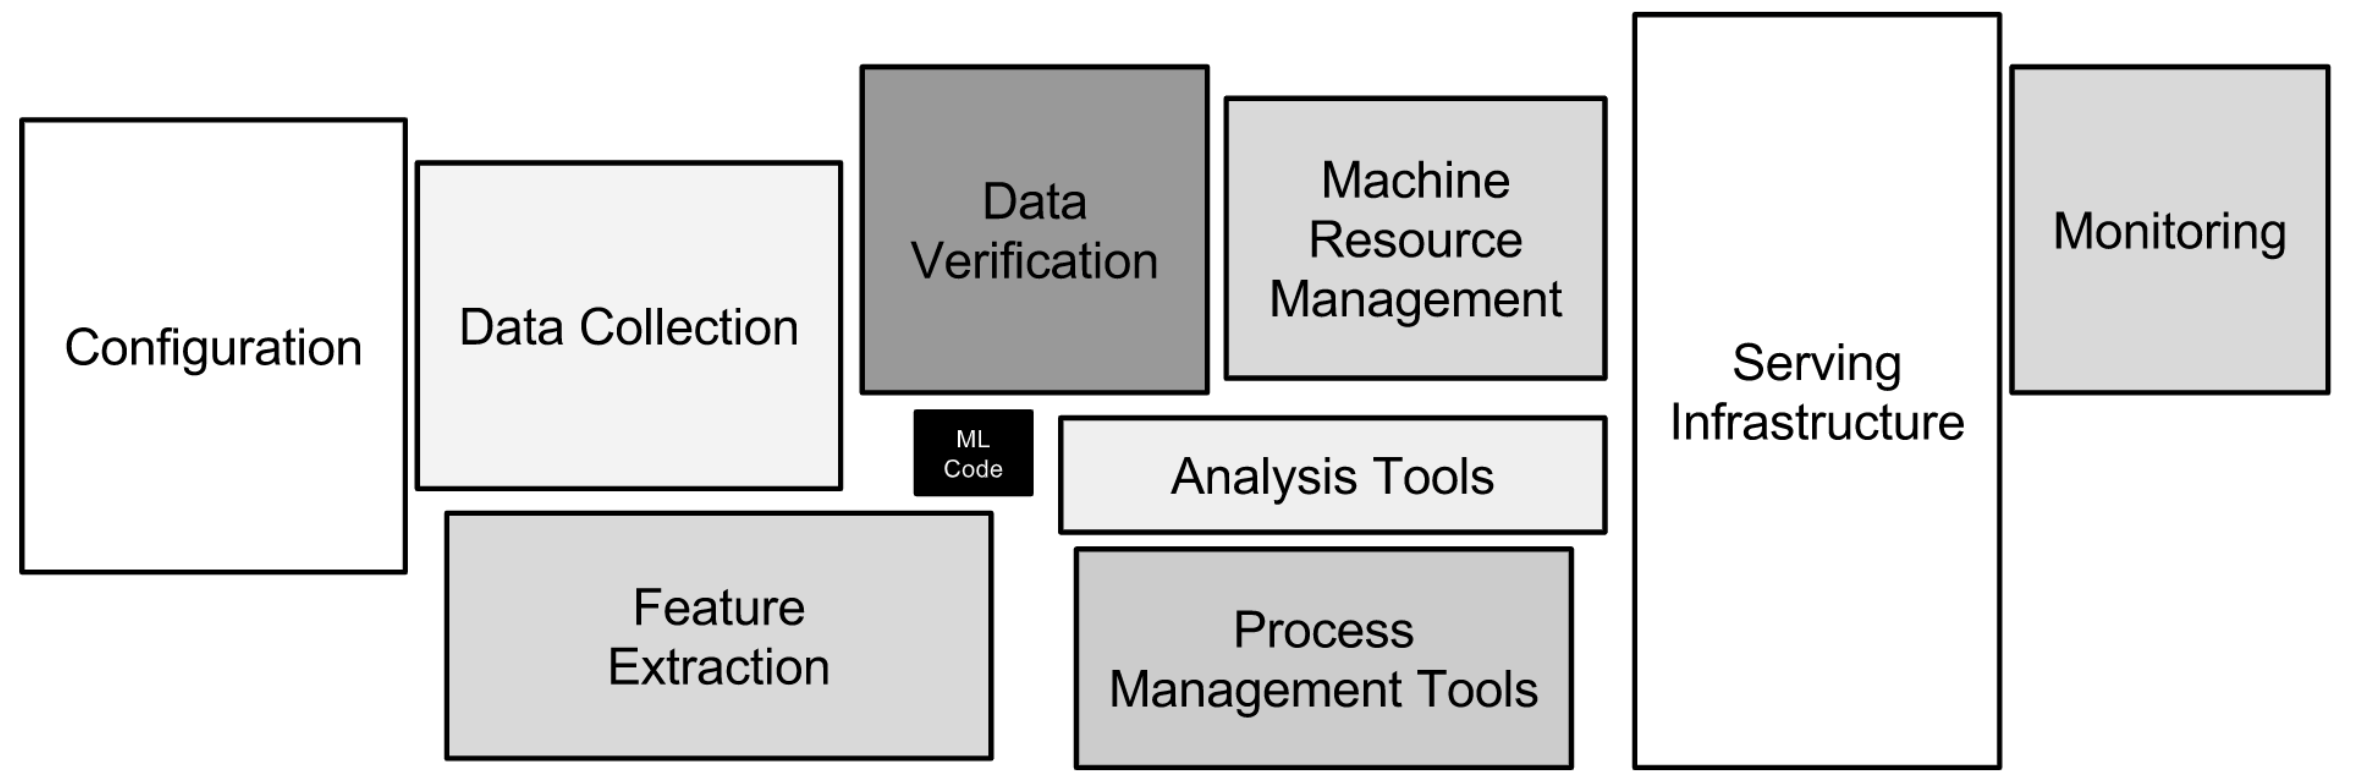
\includegraphics[width=\textwidth]{Figure/Background/sculley-googlesuite.png}
        \caption{Grandezza dei software Google AI in linee di codice, il riquadro nero rappresenta codice \textit{core AI}, i riquadri chiari invece illustrano il codice software di supporto. }
        \label{fig:sculley_googlesuite}
    \end{figure}
    \item \textbf{I software AI hanno bisogno di ingegneri del software}: Tutti i software (AI e non) hanno bisogno di installazione, configurazione, manutenzione e di pratiche che possano trasformare il codice in prodotto.
    Tim Menzies quindi definisce che il futuro dei sistemi software non può essere descritto come l'utilizzo esclusivo di una disciplina. Non può esistere solo ingegneria del software o solo intelligenza artificiale, ma, al contrario, nasceranno promettenti idee dalla combinazione di essi.\\
    \item \textbf{Una cattiva pratica di ingegneria del software implica una cattiva applicazione di AI}: Dal momento che anche l'utilizzo di AI rientra nella creazione di un software, le cattive pratiche di ingegneria del software inficiano anche sul software AI. Sculley riporta in una conferenza che i professionisti di machine learning tendono a utilizzare tutti gli attributi che sono a disposizione dai database aziendali per creare modelli predittivi. Questo comporta all'incremento di technical debt nel modello, in quanto i modelli predittivi costruiti soffrono di una stretta dipendenza con i dati aziendali e, quando sarà effettuato un cambiamento all'interno dei dati aziendali, i modelli predittivi dovranno subire aggiornamenti e manutenzione \cite{SculleyYoutube}. La violazione di principi di qualità del software, come il principio di accoppiamento e coesione, porta conseguenze anche al modello di intelligenza artificiale.
    \item \textbf{Una migliore pratica di ingegneria del software implica una migliore applicazione di AI}: Anche se non è necessariamente vero che applicare metodi di ingegneria del software può migliorare la qualità dell'applicazione AI, diversi professionisti di data science all'interno delle industrie hanno trovato estremi vantaggi nel loro utilizzo. Molti framework, come \textit{scikit-learn} \cite{scikitdoc}, forniscono diverse funzionalità orientate al riuso per avere a disposizione modelli di machine learning e metodi di ingegneria del software (ossia continuos integration, cloud-based testing).
    \item \textbf{Gli ingegneri del software hanno bisogno di particolari tipologie di AI}: Spesso i software di analisi dei dati utilizzano gli algoritmi di AI senza entrare nel dettaglio delle scelte di design del determinato tool. Novielli et al. \cite{NovielliNLP} evidenziano che molti modelli utilizzati nel campo dell'ingegneria del software volti a effettuare \textit{sentiment-analysis} sono costruiti su dati che non sono relativi al dominio d'interesse.
    Questo comporta gravi problemi in termini di performance del modello.
    Quindi, quello che sono considerati tool AI "generali", sono in realtà ristretti all'utilizzo nel dominio in cui sono stati addestrati. Gli ingegneri del software devono utilizzare quindi particolari tipologie di tool AI che siano il più possibile adatte al problema da affrontare.
    
\end{enumerate}

\subsection{Ciclo di vita di un applicazione di machine learning}
Come già definito, le applicazioni di intelligenza artificiale, dato la sua estrema importanza nel campo industriale, si sono evolute in sistemi di larga scala. Questo ha portato un'aumento della complessità di gestione dei determinati sistemi. Uno dei contributi principali che forniscono le pratiche di ingegneria del software alle applicazioni AI è la gestione del ciclo di vita.
Uno dei modelli maggiormente utilizzati è il CRISP-DM (Cross Industry Standard Process for Data Mining) \cite{crispdmWirth}, il quale scopo è di fornire alla comunità scientifica un modello affidabile e efficiente che supporti per ogni fase le applicazioni data-intensive.
Il ciclo di vita è suddiviso quindi in sei fasi, come mostrato in Figura \ref{fig:crisp_dm_process}.
I collegamenti interni del processo identificano le interazioni tra le diverse fasi del progetto e, a seconda dell'output di ogni fase, si decide la successiva fase da eseguire.
I collegamenti esterni esplicitano come il modello ha una natura ciclica. Alla fine dell'esecuzione delle 6 fasi, ovvero successivamente alla fase di deployment del modello, è possibile ricevere dall'ambiente nuovi eventi che scaturiscono la necessità di implementare ulteriori requisiti di business.
\begin{figure}[h]
    \centering
    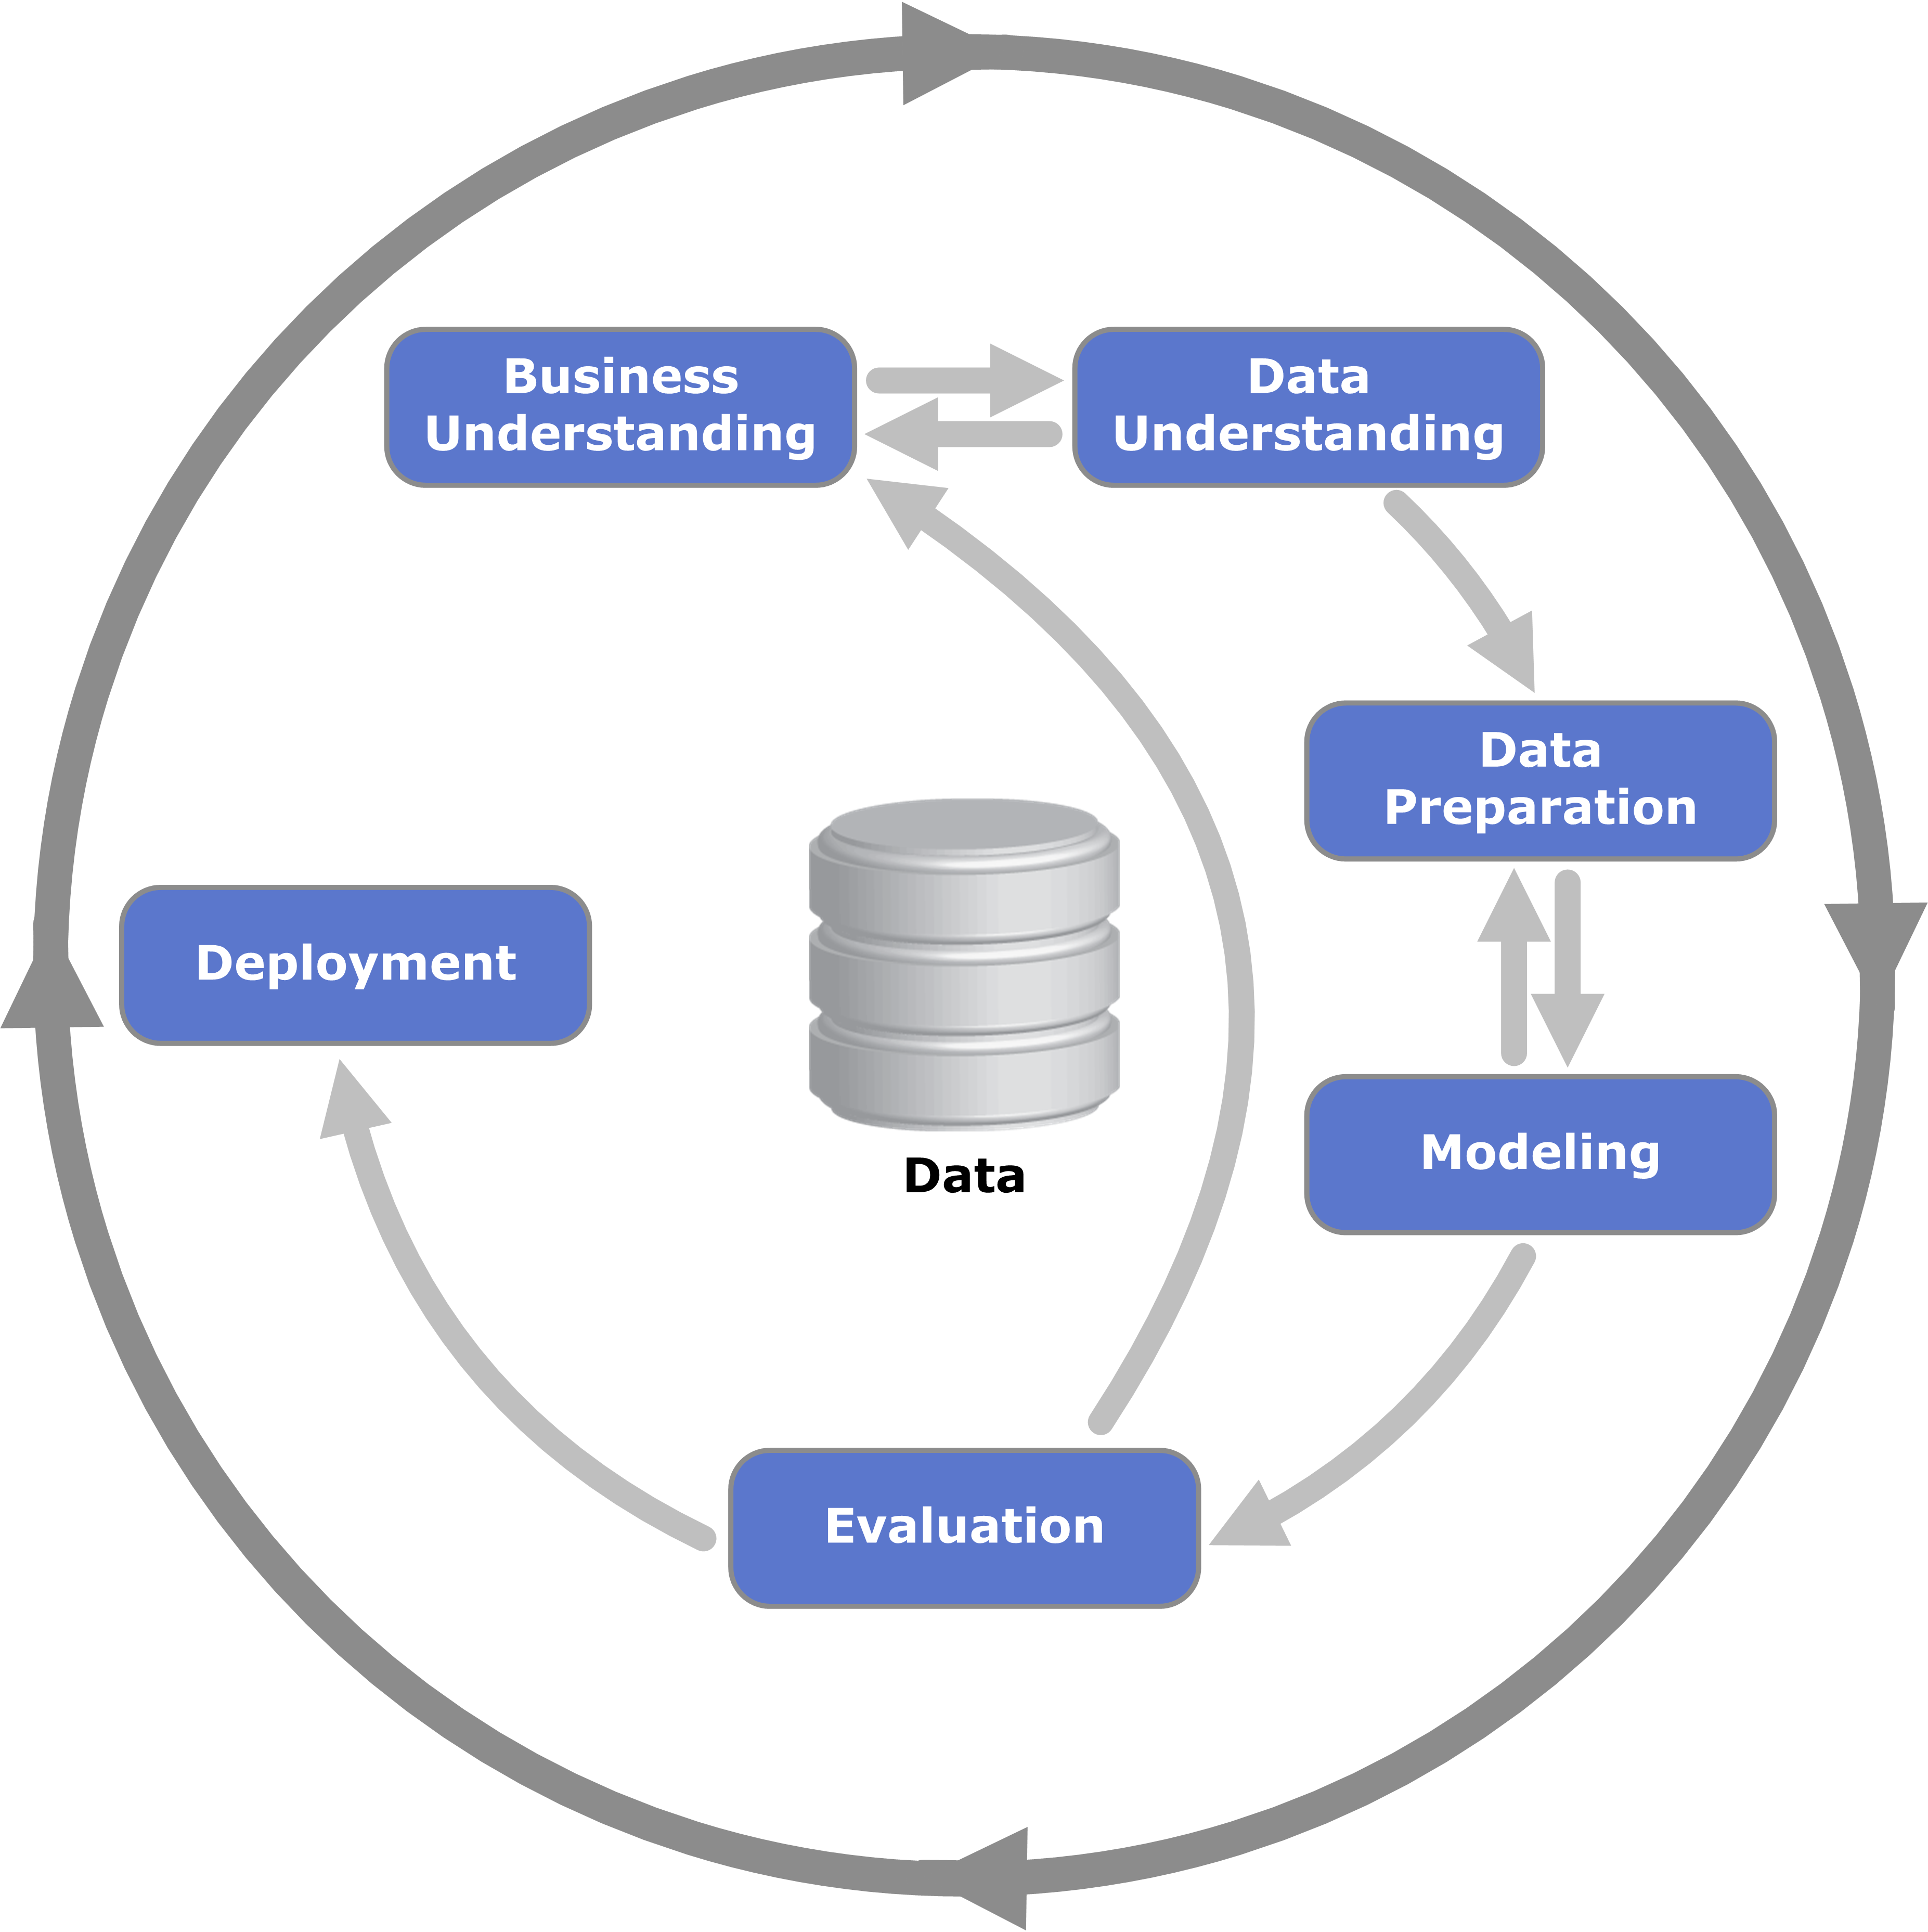
\includegraphics[width=0.5\textwidth]{Figure/Background/CRISP-DM_Process_Diagram.png}
    \caption{Processo di gestione del ciclo di vita CRISP-DM}
    \label{fig:crisp_dm_process}
\end{figure}

Le sei fasi del processo del ciclo di vita CRISP-DM sono definite in:
\begin{itemize}
    \item Business Understanding: Questa fase iniziale ha lo scopo di estrarre gli obiettivi e i requisiti del progetto da un punto di vista commerciale. La conoscenza risultante sarà poi convertita nella definizione di un problema specifico sui dati e infine sarà definita una pianificazione del progetto per raggiungere gli obiettivi.
    \item Data Understanding: Questa fase prevede la collezione dei dati e procede con le attività allo scopo di poter comprendere il dominio su cui si sta procedendo. Saranno quindi identificati problemi di qualità e saranno estratte le informazioni utili al raggiungimento degli obiettivi.
    \item Data Preparation: Questa fase prevede tutte le attività utili alla trasformazioni di un insieme di dati grezzi alla costruzione del dataset finale. Tipiche attività riguardanti la fase di data preparation sono la pulizia dei dati, la selezione degli attributi e la ristrutturazione dei dati.
    \item Modeling: In questa fase diverse tecniche per la creazione di modelli sono selezionate e applicate. Inoltre viene effettuata una configurazione dei parametri del modello al fine di ritrovare i loro valori ottimali e massimizzare le performance del modello.
    \item Evaluation: Una volta che il modello è stato costruito, è importante andare a valutare l'output della fase precedente e revisionare ogni fase del modello, al fine di poter validare che gli obiettivi definiti sono stati raggiunti. Lo scopo è quindi quello di identificare che gli obiettivi di business e i requisiti di qualità siano stati rispettati.
    \item Deployment: L'ultima fase ha come scopo quello di rendere il modello utilizzabile dagli utenti. In questa fase quindi saranno definite la serie di azioni utili a effettuare la distribuzione, l'organizzazione e la presentazione del modello. 
\end{itemize}

%%da aggiungere MLOps
